\section{RFC-0005: Proof of Relay}\label{rfc-0005-proof-of-relay}

\begin{itemize}
\tightlist
\item
  \textbf{RFC Number:} 0005
\item
  \textbf{Title:} Proof of Relay
\item
  \textbf{Status:} Implementation
\item
  \textbf{Author(s):} Lukas Pohanka (@NumberFour8), Qianchen Yu
  (@QYuQianchen)
\item
  \textbf{Created:} 2025/04/02
\item
  \textbf{Updated:} 2025/08/28
\item
  \textbf{Version:} v0.9.0 (Draft)
\item
  \textbf{Supersedes:} N/A
\item
  \textbf{Related Links:}
  \href{../RFC-0002-mixnet-keywords/0002-mixnet-keywords.md}{RFC-0002},
  \href{../RFC-0004-hopr-packet-protocol/0004-hopr-packet-protocol.md}{RFC-0004}
\end{itemize}

\subsection{1. Abstract}\label{1-abstract}

This RFC describes the structures and protocol for establishing a Proof
of Relay (PoR) of HOPR packets sent between two peers over a relay. In
addition, such PoR can be used to unlock incentives for the node
relaying the packets to the destination.

\subsection{2. Motivation}\label{2-motivation}

This RFC aims to solve the assurance of packet delivery between two
peers inside a mixnet. In particular, when data are sent from a sender
(peer A) using node B as a relay node to deliver the packet to the
destination node C, the assurance is established that:

\begin{enumerate}
\def\labelenumi{\arabic{enumi}.}
\tightlist
\item
  node A has guarantees that node B delivered A\textquotesingle s
  packets to node C
\item
  after successful relaying to C, node B possesses a cryptographic proof
  of the delivery
\item
  node B can use such proof to claim a reward from node A
\item
  the identity of node A is not revealed to node C
\end{enumerate}

\subsection{3. Terminology}\label{3-terminology}

This document builds upon standard terminology established in
\href{../RFC-0002-mixnet-keywords/0002-mixnet-keywords.md}{RFC-0002}.
Mentions to "HOPR packets" or "mixnet packets" refer to a particular
structure (\texttt{HOPR\_Packet}) defined in
\href{../RFC-0004-hopr-packet-protocol/0004-hopr-packet-protocol.md}{RFC-0004}.

In addition, this document also uses the following terms:

\begin{itemize}
\tightlist
\item
  \textbf{Channel (or Payment channel)}: a unidirectional directed
  relation of two parties (source node and destination node) that holds
  a monetary balance, that can be paid out by source to the destination,
  if certain conditions are met.
\item
  \textbf{Ticket}: a structure that holds cryptographic material
  allowing probabilistic fund transfer within the Payment channel.
\item
  \textbf{domainSeparator}: To prevent replay attacks across different
  domains (e.g., contracts, chains) where the ledger that stores channel
  states MAY be deployed, all cryptographic signatures in the HOPR
  protocol are bound to a specific execution context using a domain
  separator.
\item
  \textbf{Notice period (T\_closure)}: Minimum elapsed time required for
  an outgoing channel to transit from \texttt{PENDING\_TO\_CLOSE} to
  \texttt{CLOSED}
\end{itemize}

The above terms are formally defined in the following sections.

The key words "MUST", "MUST NOT", "REQUIRED", "SHALL", "SHALL NOT",
"SHOULD", "SHOULD NOT", "RECOMMENDED", "MAY", and "OPTIONAL" in this
document are to be interpreted as described in
\href{https://datatracker.ietf.org/doc/html/rfc2119}{IETF RFC 2119}.

\subsubsection{3.1. Cryptographic and security
parameters}\label{31-cryptographic-and-security-parameters}

This document makes use of certain cryptographic and mathematical terms.
A security parameter \texttt{L} is chosen, and corresponding
cryptographic primitives are used in a concrete instantiation of this
RFC. The specific instantiation of the current version of this protocol
is given in Appendix 1.

The security parameter \texttt{L} SHALL NOT be less than 2\^{}128 -
meaning the chosen cryptographic primitives instantiations below SHALL
NOT have less than 128-bits of security.

\begin{itemize}
\tightlist
\item
  \textbf{EC group} refers to a specific elliptic curve \texttt{E} group
  over a finite field, where computational Diffie-Hellman problem is AT
  LEAST as difficult as the chosen security parameter \texttt{L}. The
  elements of the field are denoted using lower-case letter, whereas the
  elements (also referred to as elliptic curve points, or EC points) of
  the EC group are denoted using upper-case letters.
\item
  \textbf{MUL(a,B)} represents a multiplication of an EC point
  \texttt{B} by a scalar \texttt{a} from the corresponding finite field.
\item
  \textbf{ADD(A,B)} represents an addition of two EC points \texttt{A}
  and \texttt{B} from the corresponding finite field.
\item
  \textbf{Public key} refers to a non-identity EC group element (or its
  equivalent) of a large order.
\item
  \textbf{Private key} refers to a scalar from a finite field of the
  chosen EC group. It represents a private key for a certain public key.
\item
  \textbf{Hash \texttt{H(x)}} refers to a cryptographic hash function
  taking an input of any size, and returning a fixed length output.
  Security of \texttt{H} against cryptographic attacks SHALL NOT be less
  than \texttt{L}.
\item
  \textbf{Verifiable Random Function (VRF)} produces a pseudo-random
  value that is publicly verifiable but cannot be forged or precomputed.
\end{itemize}

Nodes and clients MUST implement handling for each of the above to
ensure compliance and fault tolerance within the HOPR PoR protocol.

The concrete choices of the above cryptographic primitives for the
implementation of version 1.0 are given in Appendix 1.

\subsection{4. Payment channels}\label{4-payment-channels}

Let A, B and C be peers participating in the mixnet. Each node is in
possesion of its own private key (\texttt{Kpriv\_A}, \texttt{Kpriv\_B},
\texttt{Kpriv\_C}) and the corresponding public key (\texttt{P\_A},
\texttt{P\_B}, \texttt{P\_C}). The public keys of participating nodes
are publicly exposed.

The public keys MUST be from an elliptic curve cryptosystem represented
by an elliptic curve \texttt{E}.

Assume that node A wishes to communicate with node C, using node B as a
relay. Node A then opens a logical payment channel with node B (denoted
A -\textgreater{} B), staking some funds into this channel. Such channel
will hold the current balance and additional state information shared
between A and B and is strictly directed in the direction A
-\textgreater{} B.

For the purpose of this RFC, the amount of funds MUST be strictly
greater than 0 and MUST be strictly less than 2\^{}96.

There MUST NOT be more than a single payment channel between any two
nodes A and B in this direction. Since channel is uni-directional, there
MAY BE channel A -\textgreater{} B and also B -\textgreater{} A at the
same time.

Each channel has a unique, deterministic identifier, which is channel
ID. The channel ID for A → B MUST be computed as:
\texttt{channel\_id\ =\ H(f(P\_A)\textbar{}\textbar{}f(P\_B))} where
\texttt{\textbar{}\textbar{}} stands for byte-wise concatenation. This
construction is directional (A first, then B).

The channel MUST always be in one of the 3 logical states:

\begin{enumerate}
\def\labelenumi{\arabic{enumi}.}
\tightlist
\item
  Open
\item
  Pending to close
\item
  Closed
\end{enumerate}

Such state can be described using \texttt{ChannelStatus} enumeration:

\begin{verbatim}
ChannelStatus { OPEN, PENDING_TO_CLOSE, CLOSED }
\end{verbatim}

There is a structure called \texttt{Channel} that MUST contain at least
the following fields:

\begin{enumerate}
\def\labelenumi{\arabic{enumi}.}
\tightlist
\item
  \texttt{source}: public key of the source node (A in this case)
\item
  \texttt{destination}: public key of the destination node (beneficiary,
  B in this case)
\item
  \texttt{balance} : an unsigned 96-bit integer
\item
  \texttt{ticket\_index}: an unsigned 48-bit integer
\item
  \texttt{channel\_epoch}: an unsigned 24-bit non-zero integer
\item
  \texttt{status}: one of the \texttt{ChannelStatus} values
\end{enumerate}

\begin{verbatim}
Channel {
    source: [u8; |P_A|],
    destination: [u8; |P_B|],
    balance: u96,
    ticket_index: u48,
    channel_epoch: u24,
    status: ChannelStatus
}
\end{verbatim}

Such structure is sufficient to describe the payment channel A
-\textgreater{} B.

Channels are uniquely identified by the \texttt{channel\_id} above. The
fixed‑length byte string returned by the function is called
\texttt{ChannelId}.

\subsubsection{4.1. Payment channel
life-cycle}\label{41-payment-channel-life-cycle}

A payment channel between nodes A -\textgreater{} B MUST always be
initiated by node A. It MUST be initialized with a non-zero
\texttt{balance}, a \texttt{ticket\_index} equal to \texttt{0},
\texttt{channel\_epoch} equal to \texttt{1} and \texttt{status} equal to
\texttt{Open}. To prevent spamming, the funding \texttt{balance} MUST be
larger than \texttt{MIN\_USED\_BALANCE} and smaller than
\texttt{MAX\_USED\_BALANCE}.

In such state, the node A is allowed communicate with node C via B and
the node B can claim certain fixed amounts of \texttt{balance} to be
paid out to it in return - as a reward for the relaying work. This will
described in the later sections.

At any point in time, the channel initiator A can initiate a closure of
the channel A -\textgreater{} B. Such transition MUST change the
\texttt{status} field to \texttt{PENDING\_TO\_CLOSE} and this change
MUST be communicated to B. In such state, the node A MUST NOT be allowed
to communicate with C via B, but B MUST be allowed to still claim any
unclaimed rewards from the channel. However, B MUST NOT be allowed to
claim any rewards after \texttt{T\_closure} has elapsed since the
transition to PENDING\_TO\_CLOSE. \texttt{T\_closure} MUST be measured
in block timestamps, and both parties MUST derive it from the same
source.

After each claim is done by B, the \texttt{ticket\_index} field MUST be
incremented by 1, and such change MUST be communicated to both A and B.
The increment MAY be done by an independent trusted third party
supervising the reward claims.

The initiator A SHALL transition the channel state to \texttt{CLOSED}
(changing the \texttt{status} to \texttt{CLOSED}). Such transition MUST
NOT be possible before \texttt{T\_closure} has elapsed. The transition
MUST be communicated to B. In such state, the node A MUST NOT be allowed
to communicate with C via B, and B MUST NOT be allowed to claim any
unclaimed rewards from the channel. The \texttt{balance} in the channel
A -\textgreater{} B MUST be reset to \texttt{0} and its
\texttt{channel\_epoch} MUST be incremented by \texttt{1}.

At any point of time when the channel is at the state other than
\texttt{CLOSED}, the channel destination B MAY unilaterally transition
the channel A -\textgreater{} B to state \texttt{CLOSED}. Node B SHALL
claim unclaimed rewards before the state transition, because any
unclaimed rewards becomes unclaimable after the state transit, resulting
a lost for node B. To prevent spamming, the reward amount MUST be larger
than \texttt{MIN\_USED\_BALANCE} and smaller than
\texttt{MAX\_USED\_BALANCE}.

\subsection{5. Tickets}\label{5-tickets}

Tickets are always created by a node that is the source (\texttt{A}) of
an existing channel. It is created whenever \texttt{A} wishes to send a
HOPR packet to a certain destination (\texttt{C}), while having the
existing channel\textquotesingle s destination (\texttt{B}) act as a
relay.

Their creation MAY happen at the same time as the HOPR packet, or MAY be
precomputed in advance when usage of a certain path is known in-prior.

A Ticket:

\begin{enumerate}
\def\labelenumi{\arabic{enumi}.}
\tightlist
\item
  MUST be tied (via a cryptographic challenge) to a single HOPR packet
  (from
  \href{../RFC-0004-hopr-packet-protocol/0004-hopr-packet-protocol.md}{RFC-0004})
\item
  the cryptographic challenge MUST be solvable by the ticket recipient
  (\texttt{B}) once it delivers the corresponding HOPR packet to
  \texttt{C}
\item
  the solution of the cryptographic challenge MAY unlock a reward for
  ticket\textquotesingle s recipient \texttt{B} at expense of \texttt{A}
\item
  MUST NOT contain information about packet\textquotesingle s
  destination (\texttt{C})
\end{enumerate}

\subsubsection{5.1. Ticket structure
encoding}\label{51-ticket-structure-encoding}

The Ticket has the following structure:

\begin{verbatim}
Ticket {
    channel_id: ChannelId,
    amount: u96,
    index: u48,
    index_offset: u32,
    encoded_win_prob: u56,
    channel_epoch: u24,
    challenge: ECPoint,
    signature: ECDSASignature
}
\end{verbatim}

All multi-byte unsigned integers MUST use the big-endian encoding when
serialized.

The \texttt{ECPoint} is an encoding of an Elliptic curve point on the
chosen curve \texttt{E} that corresponds to a cryptographic challenge.
Such challenge is later solved by the ticket recipient once it forwards
the attached packet to the next downstream node.

The encoding (for serialization) of the \texttt{ECPoint} MUST be unique
and MAY be irreversible, in a sense, that the original elliptic point on
the curve \texttt{E} is not recoverable, but the encoding uniquely
identifies the said point.

The \texttt{ECDSASignature} SHOULD use the
\href{https://eips.ethereum.org/EIPS/eip-2098}{ERC-2098 encoding}, the
public key recovery bit is stored in the most significant bit of the
\texttt{s} value (which is guaranteed to be unused). Both \texttt{r} and
\texttt{s} use big-endian encoding when serialized.

\begin{verbatim}
ECDSASignature {
    r: u256
    s: u256
}
\end{verbatim}

The ECDSA signature of the ticket MUST be computed over the
\href{https://eips.ethereum.org/EIPS/eip-712}{EIP‑712} hash
\texttt{H\_ticket} of the \texttt{Ticket} typed‑data using
\texttt{domainSeparator} (\texttt{dst}):

\begin{verbatim}
H_1 = H(channel_id || amount || index || index_offset || channel_epoch || encoded_win_prob || challenge)
H_2 = H(0xfcb7796f00000000000000000000000000000000000000000000000000000000 || H_1)`
H_ticket = H(0x1901 || dst || H_2)
\end{verbatim}

The \texttt{Ticket} signature MUST be done over the same elliptic curve
\texttt{E} using the private key of the ticket creator (issuer).

\subsubsection{5.2. Construction of Proof-of-Relay (PoR)
secrets}\label{52-construction-of-proof-of-relay-por-secrets}

This section uses terms defined in Section 2.2 in
\href{../RFC-0004-hopr-packet-protocol/0004-hopr-packet-protocol.md}{RFC-0004},
namely the \texttt{SharedSecret\_i} generated for \texttt{i}-th node on
the path (\texttt{i} ranges from 0 (sender node) up to \texttt{n}
(destination node), i.e. \texttt{n} is equal to the path length). Note,
that for 0-hop path (a direct packet from sender to destination),
\texttt{n} = 1.

In the PoR mechanism, a cryptographic secret is established between
relay nodes and their adjacent nodes on the route.

Upon packet creation, the Sender node creates two structures:

\begin{enumerate}
\def\labelenumi{\arabic{enumi}.}
\tightlist
\item
  the list of \texttt{ProofOfRelayString\_i} for each \texttt{i}-th node
  on the path for i \textgreater{} 0 up to \texttt{n-1}. For
  \texttt{n=1}, the list will be empty
\item
  the \texttt{ProofOfRelayValues} structure
\end{enumerate}

Each \texttt{ProofOfRelayString\_i} contains the \texttt{challenge} for
the ticket for node the \texttt{i+1}-th and the \texttt{hint} value fort
the same node. The \texttt{hint} value is later used by the
\texttt{i+1}-th node to validate that the \texttt{challenge} is not
bogus, before it delivers the packet to the next hop.

Due to this later verification, the \texttt{hint} MUST use an encoding
useful for EC group computations on \texttt{E} (here denoted as
\texttt{RawECPoint}).

\begin{verbatim}
ProofOfRelayString_i {
    challenge: ECPoint,
    hint: RawECPoint
}
\end{verbatim}

The \texttt{ProofOfRelayValues} structure contains the
\texttt{challenge} and \texttt{hint} to the first relayer on the path,
plus it MUST contain information about the path length. This information
is later used to set the correct price of the first ticket.

Path length MUST be always less than 4 (i.e. maximum 3 hops).

\begin{verbatim}
ProofOfRelayValues {
    challenge: ECPoint,
    hint: RawECPoint,
    path_len: u8
}
\end{verbatim}

\paragraph{5.2.1. Creation of Proof of Relay strings and
values}\label{521-creation-of-proof-of-relay-strings-and-values}

Let \texttt{HS} be the Hash to Field operation defined in
\href{../RFC-0004-hopr-packet-protocol/0004-hopr-packet-protocol.md}{RFC-0004}
over the field of the chosen \texttt{E}.

The generation process of \texttt{ProofOfRelayString\_i} proceeds as
follows for each \texttt{i} from 0 to \texttt{n-1} :

\begin{enumerate}
\def\labelenumi{\arabic{enumi}.}
\item
  The \texttt{SharedKey\_i+1\_ack} is derived from the shared secret
  (\texttt{SharedSecret\_i}) provided during the HOPR packet
  construction. \texttt{SharedKey\_i+1\_ack} denotes the secret
  acknowledgement key for the next downstream node (\texttt{i+1}).

  \begin{itemize}
  \tightlist
  \item
    if \texttt{i} \textless{} \texttt{n} :
    \texttt{SharedKey\_i+1\_ack\ =\ HS(SharedKey\_i,\ "HASH\_KEY\_ACK\_KEY")}
  \item
    if \texttt{i} = \texttt{n} : the \texttt{SharedKey\_i+1\_ack} MUST
    be generated as a uniformly random byte-string with the byte-length
    of \texttt{E}\textquotesingle s field elements.
  \end{itemize}
\item
  The own shared secret \texttt{SharedKey\_i\_own} from
  \texttt{SharedSecret\_i} is generated as:
  \texttt{SharedKey\_i\_own\ =\ HS(SharedKey\_i,\ "HASH\_KEY\_OWN\_KEY")}
\item
  The \texttt{hint} value is computed:

  \begin{itemize}
  \tightlist
  \item
    if \texttt{i} = 0:
    \texttt{hint\ =\ HS(SharedKey\_0,\ "HASH\_KEY\_ACK\_KEY})
  \item
    if \texttt{i} \textgreater{} 0:
    \texttt{hint\ =\ SharedKey\_i+1\_ack} (from step 1)
  \end{itemize}
\item
  For \texttt{i} \textgreater{} 0, the \texttt{ProofOfRelayString\_i} is
  composed and added to the list:

  \begin{itemize}
  \tightlist
  \item
    \texttt{challenge} is computed as:
    \texttt{challenge\ =\ MUL(SharedKey\_i\_own\ +\ SharedKey\_i+1\_ack,\ G)}
    and encoded as \texttt{ECPoint}
  \item
    \texttt{hint} is used from step 3.
  \end{itemize}
\item
  For \texttt{i} = 0, the \texttt{ProofOfRelayValues} is created:

  \begin{itemize}
  \tightlist
  \item
    \texttt{challenge} is computed as:
    \texttt{challenge\ =\ MUL(SharedKey\_i\_own\ +\ SharedKey\_i+1\_ack,\ G)}
    and encoded as \texttt{ECPoint}
  \item
    \texttt{hint} is used from step 3.
  \item
    \texttt{path\_length} is set to \texttt{n}
  \end{itemize}
\end{enumerate}

\subsubsection{5.3 Creation of the ticket for the first
relayer}\label{53-creation-of-the-ticket-for-the-first-relayer}

The first ticket MUST be created by the packet Sender and MUST contain
the \texttt{challenge} field equal to the \texttt{challenge} in the
\texttt{ProofOfRelayValues} from the previous step.

\paragraph{\texorpdfstring{Multi-hop ticket: for \texttt{n}
\textgreater{}
1}{Multi-hop ticket: for n \textgreater{} 1}}\label{multi-hop-ticket-for-n--1}

In this situation, the \texttt{Channel} between the Sender and the next
hop MUST exist and be in the \texttt{OPEN} state.

\begin{enumerate}
\def\labelenumi{\arabic{enumi}.}
\item
  The field \texttt{channel\_id} MUST be set according to the
  \texttt{Channel} leading from the Sender to the first packet relayer.
\item
  The \texttt{amount} field SHOULD be set according to an expected
  packet price times the number of hops on the path (that is \texttt{n}
  - 1).
\item
  The \texttt{index} field MUST be set to the \texttt{ticket\_index} + 1
  from the corresponding \texttt{Channel}.
\item
  The \texttt{index\_offset} MUST be set to 1 in the current
  implementation.
\item
  The \texttt{encoded\_win\_prob} SHOULD be set according to expected
  ticket winning probability in the network.
\item
  The \texttt{channel\_epoch} MUST be set to the \texttt{channel\_epoch}
  from the corresponding \texttt{Channel}.
\end{enumerate}

\paragraph{\texorpdfstring{Zero-hop ticket: \texttt{n} =
1}{Zero-hop ticket: n = 1}}\label{zero-hop-ticket-n--1}

This is a specific case when the packet is 0-hop (\texttt{n} = 1, it is
sent directly from the Sender to the Recipient). If the \texttt{Channel}
between the Sender and Recipient does exist, it MUST be ignored.

The \texttt{Ticket} is still created:

\begin{enumerate}
\def\labelenumi{\arabic{enumi}.}
\item
  The \texttt{channel\_id} MUST be set to
  \texttt{H(P\_S\ \textbar{}\textbar{}\ P\_R)} where \texttt{P\_S} and
  \texttt{P\_R} are public keys (or their encoding) of Sender and
  Recipient respectively.
\item
  The \texttt{amount}, \texttt{index} and \texttt{channel\_epoch} MUST
  be 0
\item
  The \texttt{index\_offset} MUST be 1
\item
  The \texttt{encoded\_win\_prob} MUST be set to a value equivalent to
  the 0 winning probability
\end{enumerate}

In any case, once the \texttt{Ticket} structure is complete, it MUST be
signed by the Sender, who MUST be always the first
ticket\textquotesingle s issuer.

As described in Section 2.5 in
\href{../RFC-0004-hopr-packet-protocol/0004-hopr-packet-protocol.md}{RFC-0004},
the complete encoded \texttt{Ticket} structure becomes part of the
outgoing \texttt{HOPR\_Packet}.

\subsubsection{5.4. Ticket processing at a
node}\label{54-ticket-processing-at-a-node}

This is inherently part of the packet processing from the
\href{../RFC-0004-hopr-packet-protocol/0004-hopr-packet-protocol.md}{RFC-0004}.
Once a node receives a \texttt{HOPR\_Packet} structure, the
\texttt{Ticket} is separated and its processing is a two step process:

\begin{enumerate}
\def\labelenumi{\arabic{enumi}.}
\tightlist
\item
  The ticket is pre-verified (this is already mentioned in section 4.4
  of RFC 0003).
\item
  If the packet is to be forwarded to a next node, the ticket MUST be
  fully-verified

  \begin{itemize}
  \tightlist
  \item
    If successful, the ticket is replaced with a new ticket in the
    \texttt{HOPR\_Packet} for the next hop
  \end{itemize}
\end{enumerate}

\paragraph{5.4.1. Ticket
pre-verification}\label{541-ticket-pre-verification}

Failure to validate in any of the verification steps MUST result in
discarding the ticket and the corresponding \texttt{HOPR\_Packet}, and
interrupting the processing further.

If the extracted \texttt{Ticket} structure cannot be deserialized, the
corresponding \texttt{HOPR\_Packet} MUST be discarded. It the
\texttt{Ticket} has been issued for an unknown channel, or it does not
correspond to the channel between the packet sender and the node where
it is being processed, or the channel is in the \texttt{CLOSED} state,
the corresponding \texttt{HOPR\_Packet} MUST be discarded.

At this point, the node knows its \texttt{SharedSecret\_i} with which it
is able to decrypt the \texttt{HOPR\_Packet} and the
\texttt{ProofOfRelayString\_i} has already been extracted from the
packet header (see section 4.2 in
\href{../RFC-0004-hopr-packet-protocol/0004-hopr-packet-protocol.md}{RFC-0004}).

\begin{enumerate}
\def\labelenumi{\arabic{enumi}.}
\tightlist
\item
  \texttt{SharedSecret\_i} is used to derive
  \texttt{SharedSecret\_i\_own} as per Section 4.2.1
\item
  The \texttt{hint} is extracted from the \texttt{ProofOfRelayString\_i}
\item
  Compute \texttt{challenge\_check\ =\ ADD(SharedSecret\_i\_own,\ hint)}
\item
  The \texttt{HOPR\_Packet} MUST be rejected if encoding of
  \texttt{challenge\_check} does not match \texttt{challenge} from the
  \texttt{Ticket}
\end{enumerate}

If the pre-verification fails at any point, it still applies that the
discarded \texttt{HOPR\_Packet} MUST be acknowledged (as per section
4.2.3.1).

\paragraph{5.4.2. Ticket validation and
replacement}\label{542-ticket-validation-and-replacement}

Let \texttt{corr\_channel} be the \texttt{Channel} that corresponds to
the \texttt{channel\_id} on the \texttt{Ticket}. This channel MUST exist
and not be in the \texttt{CLOSED} state per previous section, otherwise
the entire \texttt{HOPR\_Packet} has been discarded.

If the packet is to be forwarded (as per section 4.3.1 in
\href{../RFC-0004-hopr-packet-protocol/0004-hopr-packet-protocol.md}{RFC-0004}),
the \texttt{Ticket} MUST be verified as follows:

\begin{enumerate}
\def\labelenumi{\arabic{enumi}.}
\tightlist
\item
  the \texttt{signature} of the \texttt{Ticket} is verified - if the
  signature uses ERC-2098 encoding, the ticket issuer from the signature
  is recovered and compared to the public key of the packet sender (or
  its representation)
\item
  the \texttt{amount} MUST be checked, so that it is greater than some
  given minimum ticket amount (this SHOULD be done with respect to the
  path position)
\item
  the \texttt{channel\_epoch} on the \texttt{Ticket} MUST be the current
  epoch of the \texttt{corr\_channel}.
\item
  if MUST be checked that the packet sender has enough funds to cover
  the \texttt{amount} of the ticket
\end{enumerate}

Once the above verifications have passed, verified ticket is stored as
\emph{unaknowledged} by the node and SHOULD be indexed by \texttt{hint}.
The stored unaknowledged tickets are dealt with later (see 4.2.3).

A new \texttt{Ticket} for the packet forwarded to the next hop MUST be
created.

The \texttt{HeaderPrefix} from the packet header contains the current
path position, this information is further used to determine which type
of ticket to create.

The path position is used to derive the number of remaining hops.

If the number of remaining hops is \textgreater{} 1, it MUST be checked
if a \texttt{Channel} for the next hop exists from the current node, and
if it is in the \texttt{OPEN} state. If not, the corresponding
\texttt{HOPR\_Packet} is discarded and the process is interrupted.

The process of \texttt{Ticket} creation from section 4.3 then applies,
either with the \texttt{Channel} as the next hop channel in a multi-hop
ticket (if the number of remaining hops \textgreater{} 1), or creates a
zero-hop ticket if the number of remaining hops is 1.

The following applies in addition to 4.3:

\begin{itemize}
\tightlist
\item
  the \texttt{amount} on the ticket in the multi-hop case MAY be
  adjusted (typically \texttt{amount} from previous ticket is diminished
  by the packet price)
\item
  the \texttt{challenge} MUST be set to \texttt{challenge} from the
  \texttt{ProofOfRelayString\_i} extracted from the
  \texttt{HOPR\_Packet}
\end{itemize}

If the ticket validation fails at any point, it still applies that the
discarded \texttt{HOPR\_Packet} MUST be acknowledged (as per section
4.2.3.1).

\paragraph{5.2.3. Ticket
acknowledgement}\label{523-ticket-acknowledgement}

The following sections first describe how acknowledgements are created
when sent back to the original packet\textquotesingle s Sender, and
secondly how a received acknowledgement should be processed.

\subparagraph{5.2.3.1. Sending
acknowledgement}\label{5231-sending-acknowledgement}

Per section 4.3.3 in
\href{../RFC-0004-hopr-packet-protocol/0004-hopr-packet-protocol.md}{RFC-0004},
each packet without \texttt{NoAckFlag} set MUST be acknowledged. Such an
acknowledgement becomes a payload of a 0-hop packet sent from the
original packet\textquotesingle s recipient to the original
packet\textquotesingle s sender.

\begin{verbatim}
Acknowledgement {
    ack_secret: ECScalar,
    signature: ECDSASignature
}
\end{verbatim}

There are two possibilities how the \texttt{ack\_secret} field is
calculated:

\begin{enumerate}
\def\labelenumi{\arabic{enumi}.}
\tightlist
\item
  if the \texttt{HOPR\_Packet} being acknowledged has been successfully
  processed (along with successfully validated ticket), the
  \texttt{ack\_secret} MUST be calculated as:
\end{enumerate}

\texttt{ack\_secret\ =\ HS(SharedSecret\_i,\ "HASH\_KEY\_ACK\_KEY")}

This EC field element MUST be encoded as a big-endian integer (denoted
as \texttt{ECScalar}).

\begin{enumerate}
\def\labelenumi{\arabic{enumi}.}
\setcounter{enumi}{1}
\tightlist
\item
  if the processing of the \texttt{HOPR\_Packet} failed for any reason
  (either failure of the packet processing in
  \href{../RFC-0004-hopr-packet-protocol/0004-hopr-packet-protocol.md}{RFC-0004}
  or during packet pre-verification or validation from Section 4.4):
  \texttt{ack\_secret} is set to a randomly EC point on \texttt{E}.
\end{enumerate}

This \texttt{signature} field contains the signature of the encoded
\texttt{ack\_secret} bytes. The signature done over
\texttt{H(ack\_secret)} using the private key of the acknowledging
party. For this purpose the same EC cryptosystem for signing and
verification as with \texttt{Ticket} SHOULD be used. The same encoding
of the \texttt{signature} field is used as with the \texttt{Ticket}.

\subparagraph{5.2.3.2. Receiving an
acknowledgement}\label{5232-receiving-an-acknowledgement}

After the \texttt{Ticket} has been extracted and validated by the relay
node, it awaits until the packet acknowledgement is received back from
the next hop. The node SHOULD discard tickets that
haven\textquotesingle t been acknowledged for a certain given period of
time.

Once an \texttt{Acknowledgement} is received the node MUST:

\begin{enumerate}
\def\labelenumi{\arabic{enumi}.}
\tightlist
\item
  validate the \texttt{signature} of \texttt{ack\_secret}. If invalid,
  the \texttt{Acknowledgement} MUST be discarded.
\item
  decode \texttt{ack\_secret} calculate
  \texttt{hint\ =\ MUL(ack\_secret,\ G)}
\end{enumerate}

The node then searches for a previously stored \emph{unacknowledged}
\texttt{Ticket} with the corresponding \texttt{hint} as index.

\begin{itemize}
\tightlist
\item
  If a \texttt{Ticket} with corresponding \texttt{hint} is found, it
  MUST be marked as \emph{acknowledged} and the \texttt{ack\_secret} is
  then the missing part in the solution of the cryptographic challenge
  on that \texttt{Ticket} (which is corresponding to the packet that
  just has been acknowledged).
\end{itemize}

Let \texttt{SharedSecret\_i\_own} be the value from 1) in Section 4.4.1.
The \texttt{response} to the \texttt{Ticket} challenge corresponding to
the acknowledged packet is:

\texttt{response\ =\ ack\_secret\ +\ SharedSecret\_i\_own}

The response is a field element of \texttt{E}.

\begin{itemize}
\tightlist
\item
  If no matching \texttt{Ticket} was found, the received
  \texttt{Acknowledgement} SHOULD be discarded.
\end{itemize}

\subparagraph{5.2.3.3. Derivation of VRF parameters for an Acknowledged
ticket}\label{5233-derivation-of-vrf-parameters-for-an-acknowledged-ticket}

Once the ticket becomes acknowledged, the node then calculates the
\texttt{vrf\_V} value, that will be useful to determine if the ticket is
suitable for value extraction.

Let \texttt{HC(msg,\ ctx)} be a suitable Hash to Curve function for
\texttt{E}, where \texttt{msg} is an arbitrary binary message,
\texttt{ctx} is a domain separator and whose output is a point on
\texttt{E}. See Appendix 1 for a concrete choice of \texttt{HC}.

Let \texttt{P} be the ticket recipient\textquotesingle s public key in
the EC cryptosystem on \texttt{E}.

Let \texttt{a} be the corresponding private key as field element of
\texttt{E}.

The field element MUST be representable as an unsigned big-endian
integer so it could be used e.g. as an input to a hash function
\texttt{H}. Similarly, \texttt{P} MUST be representable in an
"uncompressed" form when given to a hash function as input.

Let \texttt{H\_P} be an irreversible byte-representation of \texttt{P}.

Let \texttt{H\_ticket} be the hash of a previously acknowledged ticket
as per section 4.1.

Let \texttt{R} be a sequence of 64 uniformly randomly generated bytes
using a CSPRNG.

\begin{verbatim}
B = HC(H_P || H_ticket, dst)
V = MUL(a, B)
r = HS(a || v || R, dst)
R_v = MUL(r, B)
h = HS(P || V || R_v || H_ticket)
s = r + h * a
\end{verbatim}

The \texttt{vrf\_V} is the uncompressed representation of the EC point
\texttt{V} as \texttt{X\ \textbar{}\textbar{}\ Y}, where \texttt{X} and
\texttt{Y} are big-endian unsigned integer representation of the EC
point\textquotesingle s coordinates.

\subsection{6 Ticket and Channel
interactions}\label{6-ticket-and-channel-interactions}

\subsubsection{6.1. Discovering acknowledged winning
tickets}\label{61-discovering-acknowledged-winning-tickets}

The aknowledged tickets are \emph{probabilistic} in the sense that the
monetary value represented by the \texttt{amount} MUST be claimable only
if the aknowledged ticket is \emph{winning}. This is determined using
the \texttt{encoded\_win\_prob} field on the \texttt{Ticket}.

Let \texttt{luck} be an unsigned 56-bit integer in the big endian
encoding created by truncating the output of the following hash output:

\texttt{H(H\_ticket\ \textbar{}\textbar{}\ response\ \textbar{}\textbar{}\ vrf\_V)}

The \texttt{H\_ticket} is the hash of the \texttt{Ticket} as defined in
section 4.1.

The \texttt{response} is a field element of \texttt{E} and MUST be
encoded as big-endian unsigned integer (i.e. has the same encoding as
\texttt{ECScalar}).

The \texttt{vrf\_V} is a value computed by the ticket recipient during
acknowledgement.

The \texttt{amount} on the \texttt{Ticket} MUST be claimable only if
\texttt{luck} \textless{} \texttt{encoded\_win\_prob} on the
\texttt{Ticket}. Such an acknowledged ticket is called \emph{winning}
ticket.

\subsubsection{6.2. Claiming a winning
ticket}\label{62-claiming-a-winning-ticket}

The monetary value represented by the \texttt{amount} on a
\emph{winning} ticket can be claimable at some 3rd party which provides
such service. Such a 3rd party MUST have the ability to modify global
state of all the involved \texttt{Channels}.

Such \texttt{amount} SHOULD be claimable only if the \texttt{Channel}
corresponding the winning ticket has enough \texttt{balance}
\textgreater= \texttt{amount}.

Any holder of a \emph{winning} ticket can claim the \texttt{amount} on
the ticket by submitting the following:

\begin{itemize}
\tightlist
\item
  the entire encoded \texttt{Ticket} structure of the winning ticket
\item
  \texttt{response} encoded as field element of \texttt{E}
\item
  the public key \texttt{P} of the recipient of the ticket
\item
  values \texttt{V}, \texttt{h} and \texttt{s} computed in Section
  4.2.3.3
\end{itemize}

If the 3rd party wishes to verify the claim, it proceeds as follows. If
any of the below check fails, the \texttt{amount} MUST not be claimable.

\begin{enumerate}
\def\labelenumi{\arabic{enumi}.}
\item
  Compute \texttt{H\_ticket} as per 4.1 and verify the
  ticket\textquotesingle s signature
\item
  The \texttt{Channel} matching \texttt{channel\_id} MUST exist, MUST
  NOT be \texttt{CLOSED}, its \texttt{channel\_epoch} MUST match with
  the one on the ticket and SHOULD have \texttt{balance} \textgreater=
  \texttt{amount}.
\item
  The \texttt{index} on the ticket MUST be greater or equal to
  \texttt{ticket\_index} on the \texttt{Channel}
\item
  The 3rd party applies appropriate encoding to obtain \texttt{H\_P}
  from \texttt{P}. The performs the following computations:
\end{enumerate}

\begin{verbatim}
B = HC(H_P || H_ticket, dst)
sB = MUL(s, B)
hV = MUL(h, V)
R = sB - hV
h_check = HS(P || V || R || H_ticket, dst)
\end{verbatim}

Finally, the \texttt{h\_check} MUST be equal to \texttt{h}.

\begin{enumerate}
\def\labelenumi{\arabic{enumi}.}
\setcounter{enumi}{4}
\item
  The result of \texttt{MUL(response,\ G)} MUST be equal to the
  \texttt{challenge} from the \texttt{Ticket}. If unique encoding of
  \texttt{ECPoint} was used, their encoding MAY be compared instead.
\item
  The \texttt{luck} value computed using the given \texttt{V} MUST be
  less than the \texttt{encoded\_win\_prob} from the \texttt{Ticket}
\end{enumerate}

To satisfy the claim, the 3rd party MAY also adjust the balance on a
\texttt{Channel} that is in the opposite direction of the claim (ticket
receiver -\textgreater{} ticket issuer), if such channel exist and is in
an \texttt{OPEN} state.

Upon successful redemption, the 3rd party MUST make sure that:

\begin{enumerate}
\def\labelenumi{\arabic{enumi}.}
\tightlist
\item
  The \texttt{balance} on \texttt{Channel} from which the claim has been
  made MUST be decreased by \texttt{amount}
\item
  The \texttt{ticket\_index} on \texttt{Channel} is set to
  \texttt{index} + \texttt{index\_offset} (where \texttt{index} and
  \texttt{index\_offset} are from the claimed ticket)
\end{enumerate}

\subsection{7. Appendix 1}\label{7-appendix-1}

The current implementation of the Proof of Relay protocol (which is in
correspondence with the HOPR Packet protocol from
\href{../RFC-0004-hopr-packet-protocol/0004-hopr-packet-protocol.md}{RFC-0004}):

\begin{itemize}
\item
  Hash function \texttt{H} is Keccak256
\item
  Elliptic curve \texttt{E} is chosen as secp256k1
\item
  HS is instantiated via \texttt{hash\_to\_field} using
  \texttt{secp256k1\_XMD:SHA3-256\_SSWU\_RO\_} as defined in
  \href{https://www.rfc-editor.org/info/rfc9380}{RFC-9380}
\item
  HC is instantiated via \texttt{hash\_to\_curve} using
  \texttt{secp256k1\_XMD:SHA3-256\_SSWU\_RO\_} as defined in
  \href{https://www.rfc-editor.org/info/rfc9380}{RFC-9380}
\item
  The one-way encoding \texttt{ECPoint} is done as \texttt{Keccak256(P)}
  where \texttt{P} denotes secp256k1 point in uncompressed form. The
  output of the hash has the first 12 bytes removed, which leaves the
  length at 20 bytes.
\item
  \textbf{MIN\_USED\_BALANCE} = \texttt{1e-18} HOPR.
\item
  \textbf{MAX\_USED\_BALANCE} = \texttt{1e7} HOPR.
\end{itemize}

\subsection{8. Appendix 2}\label{8-appendix-2}

This appendix describes the ticket states which are implementation
specific for the current Proof Of Relay implementation as part of the
HOPR protocol.

\begin{itemize}
\item
  \textbf{Ticket} (unsigned or signed, but not yet verified)

  \begin{itemize}
  \tightlist
  \item
    Contains all ticket fields (channel\_id, amount, index,
    index\_offset, winProb, channel\_epoch, challenge, signature).
  \item
    A Ticket without a signature MUST NOT be accepted by peers and MUST
    NOT be transmitted except for internal construction.
  \end{itemize}
\item
  \textbf{VerifiedTicket} (signed and verified)

  \begin{itemize}
  \tightlist
  \item
    The signature MUST verify against
    \texttt{get\_hash(domainSeparator)} and recover the ticket issuer's
    address.
  \item
    \texttt{verified\_hash} MUST equal
    \texttt{Ticket::get\_hash(domainSeparator)};
    \texttt{verified\_issuer} MUST equal the recovered signer.
  \end{itemize}
\item
  \textbf{UnacknowledgedTicket} (VerifiedTicket + own half-key)

  \begin{itemize}
  \tightlist
  \item
    Produced when the recipient binds its own PoR half-key to the
    VerifiedTicket while waiting for the downstream acknowledgement.
  \end{itemize}
\item
  \textbf{AcknowledgedTicket} (VerifiedTicket + PoR response)

  \begin{itemize}
  \tightlist
  \item
    Produced once the recipient learns the downstream half-key and
    reconstructs \texttt{Response}.
  \end{itemize}
\item
  \textbf{RedeemableTicket} (winning, issuer-verified, VRF-bound)

  \begin{itemize}
  \tightlist
  \item
    Produced from an AcknowledgedTicket by attaching VRF parameters
    derived with the redeemer's chain key and the
    \texttt{domainSeparator}.
  \item
    A RedeemableTicket MUST be suitable for on-chain submission.
  \end{itemize}
\item
  \textbf{TransferableWinningTicket} (wire format for
  aggregation/transfer)

  \begin{itemize}
  \tightlist
  \item
    A compact, verifiable representation of a \textbf{winning} ticket
    intended for off-chain aggregation.
  \end{itemize}
\end{itemize}

\subsubsection{8.1. Allowed transitions}\label{81-allowed-transitions}

\pandocbounded{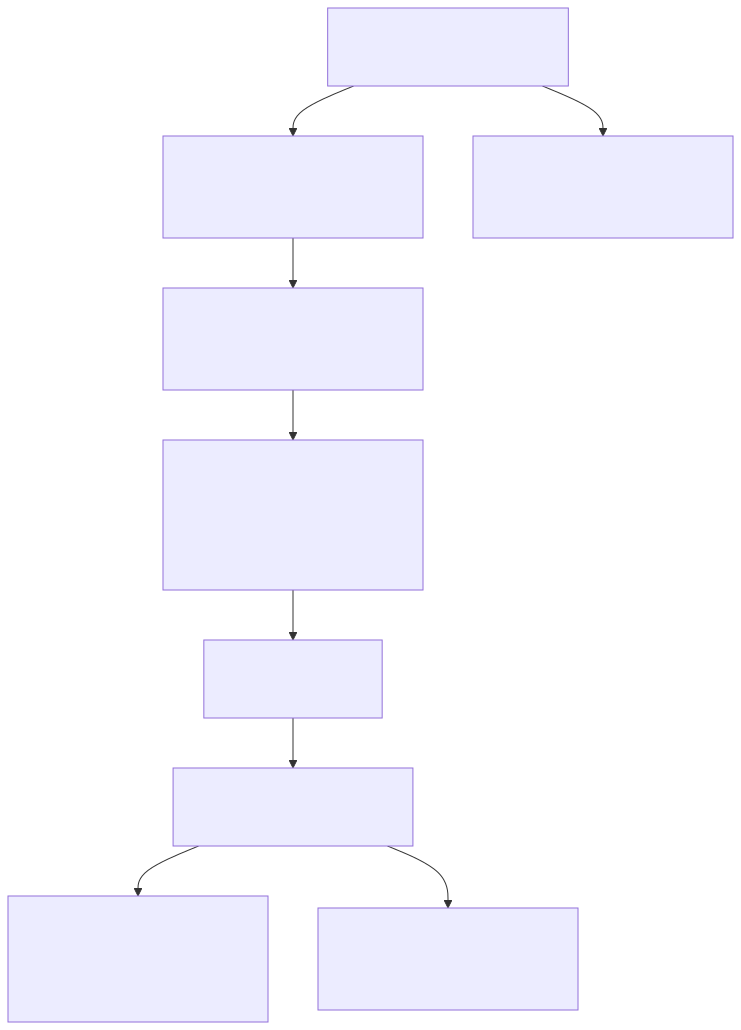
\includegraphics[keepaspectratio,width=\maxwidth,alt={Mermaid Diagram 1}]{generated/0005-proof-of-relay/mermaid_1.png}}

\begin{enumerate}
\def\labelenumi{\arabic{enumi}.}
\item
  \texttt{Ticket\ -\/-sign-\/-\textgreater{}\ VerifiedTicket}

  \begin{itemize}
  \item
    Pre-conditions:

    \begin{itemize}
    \tightlist
    \item
      Ticket MUST include all mandatory fields and satisfy bounds
      (amount ≤ 10\^{}25; index ≤ 2\^{}48; index\_offset ≥ 1;
      channel\_epoch ≤ 2\^{}24).
    \end{itemize}
  \item
    Post-conditions:

    \begin{itemize}
    \tightlist
    \item
      A valid ECDSA signature over \texttt{get\_hash(domainSeparator)}
      is attached.
    \end{itemize}
  \end{itemize}
\item
  \texttt{Ticket\ -\/-verify(issuer,\ domainSeparator)-\/-\textgreater{}\ VerifiedTicket}

  \begin{itemize}
  \tightlist
  \item
    MUST recover \texttt{issuer} from \texttt{signature} over
    \texttt{get\_hash(domainSeparator)}.
  \item
    On failure, verification MUST be rejected.
  \end{itemize}
\item
  \texttt{VerifiedTicket\ -\/-into\_unacknowledged(own\_key)-\/-\textgreater{}\ UnacknowledgedTicket}

  \begin{itemize}
  \tightlist
  \item
    Binds the recipient's PoR half-key. No additional checks REQUIRED.
  \end{itemize}
\item
  \texttt{UnacknowledgedTicket\ -\/-acknowledge(ack\_key)-\/-\textgreater{}\ AcknowledgedTicket}

  \begin{itemize}
  \tightlist
  \item
    Compute \texttt{Response\ =\ combine(own\_key,\ ack\_key)}.
  \item
    The derived challenge \texttt{Response.to\_challenge()} MUST equal
    \texttt{ticket.challenge}.
  \item
    On mismatch, the transition MUST fail with \texttt{InvalidChallenge}
    and the ticket MUST remain unacknowledged.
  \end{itemize}
\item
  \texttt{AcknowledgedTicket(Untouched)\ -\/-into\_redeemable(chain\_keypair,\ domainSeparator)-\/-\textgreater{}\ RedeemableTicket}

  \begin{itemize}
  \tightlist
  \item
    The caller (redeemer) MUST NOT be the ticket issuer (Loopback
    prevention).
  \item
    Derive VRF parameters over
    \texttt{(verified\_hash,\ redeemer,\ domainSeparator)}.
  \item
    The resulting RedeemableTicket MAY be submitted on-chain if winning
    (see §3).
  \end{itemize}
\item
  \texttt{AcknowledgedTicket(Untouched)\ -\/-into\_transferable(chain\_keypair,\ domainSeparator)-\/-\textgreater{}\ TransferableWinningTicket}

  \begin{itemize}
  \tightlist
  \item
    Equivalent to \texttt{into\_redeemable} followed by conversion to
    transferable form; retains VRF and response.
  \end{itemize}
\item
  \texttt{TransferableWinningTicket\ -\/-into\_redeemable(expected\_issuer,\ domainSeparator)-\/-\textgreater{}\ RedeemableTicket}

  \begin{itemize}
  \tightlist
  \item
    MUST verify: \texttt{signer\ ==\ expected\_issuer} and the embedded
    signature over \texttt{get\_hash(domainSeparator)}.
  \item
    MUST recompute ``win'' locally (see §3). On failure, MUST reject.
  \end{itemize}
\item
  \texttt{VerifiedTicket\ -\/-leak()-\/-\textgreater{}\ Ticket}

  \begin{itemize}
  \tightlist
  \item
    Debug/escape hatch only. Implementations SHOULD avoid downgrading
    state in production flows.
  \end{itemize}
\end{enumerate}

\subsection{9. Appendix 3}\label{9-appendix-3}

Domain separator (\texttt{dst}) for the current implementation (in
Solidity) is derived as:

\begin{verbatim}
domainSeparator = keccak256(
  abi.encode(
    keccak256("EIP712Domain(string name,string version,uint256 chainId,address verifyingContract)"),
    keccak256(bytes("HoprChannels")),
    keccak256(bytes(VERSION)),
    chainId,
    address(this)
  )
)
\end{verbatim}

\subsection{10. References}\label{10-references}
